\documentclass[11pt, oneside]{article}   	% use "amsart" instead of "article" for AMSLaTeX format
\usepackage{geometry}                		% See geometry.pdf to learn the layout options. There are lots.
\geometry{letterpaper}                   		% ... or a4paper or a5paper or ... 
%\geometry{landscape}                		% Activate for rotated page geometry
\usepackage[parfill]{parskip}    			% Activate to begin paragraphs with an empty line rather than an indent
\usepackage{graphicx}				% Use pdf, png, jpg, or eps§ with pdflatex; use eps in DVI mode
								% TeX will automatically convert eps --> pdf in pdflatex		
\usepackage{amssymb}
\usepackage{amsthm}
\usepackage{hyperref}
\usepackage{mathtools}
\usepackage{enumerate}
\usepackage{caption}  % Required for caption outside of figure
\usepackage{tikz}


\title{Homework 0 \\ CSC 277 / 477 \\ End-to-end Deep Learning \\ Fall 2024}
\author{John Doe - \texttt{jdoe@ur.rochester.edu}}
\date{}					

\begin{document}

\maketitle

\begin{center}
    \textbf{Deadline:} See Blackboard    
\end{center}


\section*{Instructions}

Your homework solution must be typed and prepared in \LaTeX. It must be output to PDF format. To use \LaTeX, we suggest using \url{http://overleaf.com}, which is free.

Your submission must cite any references used (including articles, books, code, websites, and personal communications).  All solutions must be written in your own words, and you must program the algorithms yourself. \textbf{If you do work with others, you must list the people you worked with.} Submit your solutions as a PDF to Blackboard. 


Your programs must be written in Python. The relevant code should be in the PDF you turn in. If a problem involves programming, then the code should be shown as part of the solution. One easy way to do this in \LaTeX \, is to use the verbatim environment, i.e., \textbackslash begin\{verbatim\} YOUR CODE \textbackslash end\{verbatim\}.



%%%%%%%%%%%%%%%%%%%%%%%%%%%%%%%%%%%%%%%%%%%%%

\paragraph{About Homework 0:} Homework 0 is intended to review prerequisite skills, help you become familiar with LaTeX, and ensure you have your programming environment prepared. \emph{Later assignments will be more challenging! Do not think all assignments will be this short or require little time to train networks.} Copy and paste this template into an editor, e.g., \url{www.overleaf.com}, and then just type the answers in. You can use a math editor to make this easier, e.g., CodeCogs Equation Editor or MathType. \hyperlink{https://blog.writefull.com/texgpt-harness-the-power-of-chatgpt-in-overleaf/}{You may use the AI (LLM) plugin for Overleaf for help you with \LaTeX formatting.}


%CodeCogs: \url{https://www.codecogs.com/latex/eqneditor.php}

%MathType: \url{http://www.dessci.com/en/products/mathtype/}
%For MathType, you have to tell it to export as LaTex. 


\clearpage

\section*{Problem 1 - Linear Algebra Review \#1}

Let matrix $\mathbf{A} \in \mathbb{R}^{n\times m}$ and matrix  $\mathbf{B} \in \mathbb{R}^{n \times n}$, where $n \neq m$.

\subsection*{Part 1 (1 point)}
 If it is possible to compute the matrix product $\mathbf{AB}$, give the size of the matrix produced. Otherwise, write, `Not possible.' 

\textbf{Answer:} \\
Not possible. 

\subsection*{Part 2 (1 point)}
If it is possible to compute the matrix product $\mathbf{BA}$, give the size of the matrix produced. Otherwise, write, `Not possible.' 

\textbf{Answer:} \\
The size of the matrix produced is $ n \times m $.

\clearpage

\section*{Problem 2 - Linear Algebra Review \#2}
Let  $
 {\bf{A}} = \left( {\begin{array}{*{20}r}
   0 & 0   \\
   0 & 2   \\
\end{array}} \right)
 $
and
$
 {\bf{B}} = \left( {\begin{array}{*{20}r}
   1 & 5 & 0  \\
   2 & 10 & 2  \\
\end{array}} \right)  
$
and
${\bf{D}} = \left( {\begin{array}{*{20}r}
   1 & 1 & 2 & 3 & 5 & 4 \\
   1 & 2 & 3 & 6 & 6 & 6 \\
   1 & 1 & 2 & 3 & 5 & 4 \\
   1 & 0 & 1 & 0 & 4 & 2 \\
\end{array}} \right). \\ 
$ 

Low rank approximations are used in algorithms for updating large neural networks on modest hardware. In this problem we will assess your understanding of rank in linear algebra.


\subsection*{Part 1 (1 points)}
Compute $\operatorname{rank}(\mathbf{A})$.

\textbf{Answer:} \\
$\operatorname{rank}(\mathbf{A}) = 1$.

\subsection*{Part 2 (1 points)}
Compute $\operatorname{rank}(\mathbf{B})$.

\textbf{Answer:} \\
$\operatorname{rank}(\mathbf{B}) = 2$.

\subsection*{Part 3 (1 points)}
Compute $\operatorname{rank}(\mathbf{D})$.  

\textbf{Answer:} \\
$\operatorname{rank}(\mathbf{D}) = 2$.

\subsection*{Part 4 (1 points)}
Compute $\mathbf{AB}$ and $\operatorname{rank}(\mathbf{AB})$.  

\textbf{Answer:} \\
$AB = \left( {\begin{array}{*{20}r}
    0 & 0 & 0  \\
    4 & 20 & 10  \\
 \end{array}} \right)
$

$\operatorname{rank}(\mathbf{AB}) = 1$.


\subsection*{Part 5 - Compression with linearly dependent columns (5 points)}
Now we are going to use linearly independent columns of matrix $\mathbf{D}$ to create an compressed version of matrix $\mathbf{D}$. We will use the $\mathbf{D} = \mathbf{CR}$ decomposition, i.e., rank factorization  (column-row factorization). Do the decomposition and provide $\mathbf{C} \in \mathbb{R}^{4 \times r}$ and $\mathbf{R} \in \mathbb{R}^{r \times 6}$. Calculate the compression ratio by comparing the total number of elements in original matrix and in decomposed matrices. Explain why $r$ is the rank of $\mathbf{D}$.

You may read about the CR factorization \href{https://blogs.mathworks.com/cleve/2020/10/23/gil-strang-and-the-cr-matrix-factorization/}{here} and \href{https://en.wikipedia.org/wiki/Rank_factorization}{here}. You can implement this factorization using singular value decomposition or by using reduced row echelon form.

\textbf{Answer:} \\

$\mathbf{C} = 
\left( {\begin{array}{*{20}r}
    1 & 1 \\
    1 & 2 \\
    1 & 1 \\
    1 & 0 \\
 \end{array}} \right)
$ 
\\
\textit{NOTE: C consists of the linearly independent columns of D}
\\
$\mathbf{R} =
\left( {\begin{array}{*{20}r}
    1 & 0 & 1 & 2 & 3 & 4 \\
    0 & 1 & 1 & 2 & 3 & 2 \\
 \end{array}} \right)
$
\\
\textit{NOTE: R is formed by expressing all columns of D as linear combinations of the columns in C}

Compression ratio: $\frac{24}{4 \times 2 + 2 \times 6} = \frac{24}{20} = 1.2$

The reason why $r$ is the rank of $\mathbf{D}$ is because there are only 2 linearly independent columns in D.


\clearpage


\clearpage


\section*{Problem 3 - Softmax Properties}

\subsection*{Part 1 (5 points)}
Recall the softmax function, which is the most common activation function used for the output of a neural network trained to do classification. In a vectorized form, it is given by
\begin{equation*}
\operatorname{softmax} \left( {\mathbf{a}} \right) = \frac{{\exp \left( {\mathbf{a}} \right)}}
{{\sum\nolimits_{j = 1}^K {\exp \left( {a_j } \right)} }},
\end{equation*}
where $\mathbf{a}\in \mathbb{R}^K$ and has the ``logits'' from the output layer of the network before the softmax activation function. The $\exp$ function in the numerator is applied element-wise and $a_j$ denotes the $j$'th element of $\mathbf{a}$.

Show that the softmax function is invariant to constant offsets to its input, i.e., 
\[
\operatorname{softmax} \left( {{\mathbf{a}} + {c\mathbf{1}}} \right) = \operatorname{softmax} \left( {\mathbf{a}} \right),
\]
where $c\in \mathbb{R}$ is some constant and $\mathbf{1}$ denotes a column vector of 1's.

\textbf{Solution:} \\

Consider adding a constant $c$ to each of the element in vector $\mathbf{a}$, the softmax function for $\mathbf{a} + c\mathbf{1}$ is:
\begin{proof}
    \begin{equation*}
        \operatorname{softmax} \left( {{\mathbf{a}} + {c\mathbf{1}}} \right) = \frac{\exp(\mathbf{a} + c\mathbf{1})}{\sum_{j=1}^{K}\exp(a_j + c)}
    \end{equation*}
    \\
    Since $\exp(a + c\mathbf{1})$ applies element-wise, we have:
    \begin{equation*}
        \exp(\mathbf{a} + c\mathbf{1}) = \exp(\mathbf{a}) \cdot \exp(c)
    \end{equation*}
    \\
    Thus, we can rewrite the softmax function as:
    \begin{equation*}
        \operatorname{softmax} \left( {{\mathbf{a}} + {c\mathbf{1}}} \right) = \frac{\exp(\mathbf{a}) \cdot \exp(c)}{\exp(c) \cdot \sum_{j=1}^{K}\exp(a_j)} = \frac{\exp(\mathbf{a})}{\sum_{j=1}^{K}\exp(a_j)}
    \end{equation*}
    \\
    Hence,
    \begin{equation*}
        \operatorname{softmax} \left( {{\mathbf{a}} + {c\mathbf{1}}} \right) = \operatorname{softmax} \left( {{\mathbf{a}}} \right) 
    \end{equation*}
    The softmax function is invariant to adding a constant vector to its input.
\end{proof}

%----------------------------------
\subsection*{Part 2 (3 points)}
In practice, why is the observation that the softmax function is invariant to constant offsets to its input important when implementing it in a neural network?

\textbf{Solution:} \\

The invariance of the softmax function to constant offsets is important in neural networks because:
\\
\begin{enumerate}
    \item \textbf{Numerical Stability:} Subtracting the maximum logit before applying softmax prevents overflow/underflow in the exponentials, ensuring stable computations.
    \item \textbf{Interpretability:} The relative differences between logits determine the output probabilities, making the absolute scale irrelevant and allowing focus on relative confidence between classes.
    \item \textbf{Model Flexibility:} This property permits shifts in logits (e.g., due to batch normalization) without affecting the final output, enabling more flexible model design. (i.e. due to the flexibility on ``paddings'')
\end{enumerate}

\newpage


\section*{Problem 4 - Feedforward Fully-Connected Networks (10 points)}
This class assumes that you already know neural network basics. For this problem you need to use PyTorch and/or PyTorch Lightning. PyTorch Lightning is a wrapper around PyTorch that attempts to simplify a lot of the code, enforcing best practices, and making the code more portable across hardware platforms.

In this problem you will create a neural network that will be trained on the Iris dataset for multi-class classification. We will use a 2-dimensional version of the dataset. Download \texttt{iris-train.txt} and \texttt{iris-test.txt}. Each row is one data instance. The first column is the label (1, 2 or 3) and the next two columns are features. Build up your data loading process re-arrange the dataset into a suitable format for training. 

We will train two neural networks. The first will have only the output layer, i.e., it is described by a $2 \times 3$ matrix with a bias and is a linear classifier. The second is a nonlinear classifier that will have one hidden layer with 5 units.  Use AdamW as your optimizer and use CrossEntropyLoss. Train the two network for 1000 epochs on the training dataset. Try running your code a few times with different random initializations, since you may hit a poor local optima. You should normalize the data when given to the network by subtracting the mean of the training data. You only need to report on your best run.

\begin{figure}
    \centering
    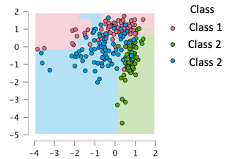
\includegraphics{example.png}
    \caption{An example decision boundary on a different dataset.}
    \label{fig:example}
\end{figure}


Please provide the following:
\begin{enumerate}
    \item Show the train loss curves in two plots for both networks (2 pts). Label one linear neural network and the other nonlinear neural network.
    \item Measure the accuracy of both networks on the testing \emph{and} training datasets (3 pts). Put this in a \LaTeX table.
    \item Create decision boundaries for both networks and show them. Make sure to label your plots. Feel free to find helper code online for displaying the decision boundary (5 pts). An example decision boundary is provided in Fig.~\ref{fig:example}. Show the training data points in the figure, and color them appropriately for their label.
    \item Provide your code for credit.
\end{enumerate}

\newpage

\textbf{Answer:} \\
\begin{center}
    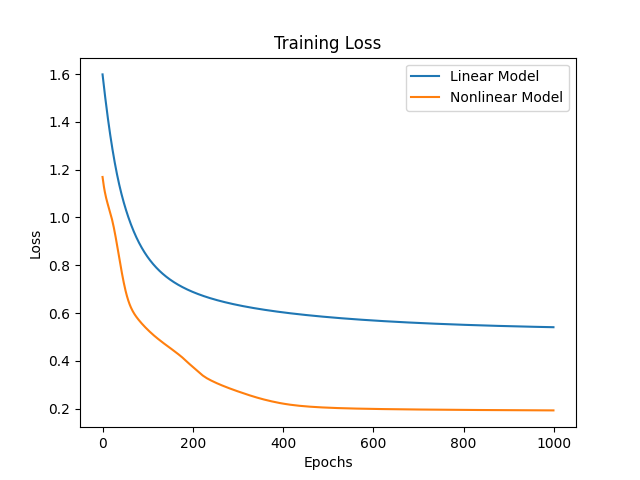
\includegraphics[width=0.5\textwidth]{Trainloss.png}
    \captionof{figure}{Train loss curves for linear neural network and nonlinear neural network}
\end{center}
\\
\begin{center}
    \begin{tabular}{|c|c|c|}
        \hline
        & Train Accuracy & Test Accuracy \\ \hline
        Linear Model & 0.90 & 0.84 \\ \hline
        Nonlinear Model & 0.92 & 0.82 \\ \hline
    \end{tabular}
    \captionof{table}{Training and Testing Accuracy of Models}
\end{center}
\\




\textbf{Code for Problem 4:} \\
\begin{verbatim}
CODE HERE
\end{verbatim}



\end{document}  